\chapter{Theory questions}

18/02/11\\

Descrivere, con l’aiuto di disegni se necessario, due tecniche per realizzare {\bf floating gate auto-allineate} nell’ambito del flusso di processo di una memoria flash.\\

\vspace{3mm}

21/10/09\\

Una opportuna crescita epitassiale di silicio, con possibilità di doping in-situ, è stata utilizzata per
ottenere il profilo di drogaggio in As mostrato in figura1 (si consideri solo il grafico in dots neri).

\centering
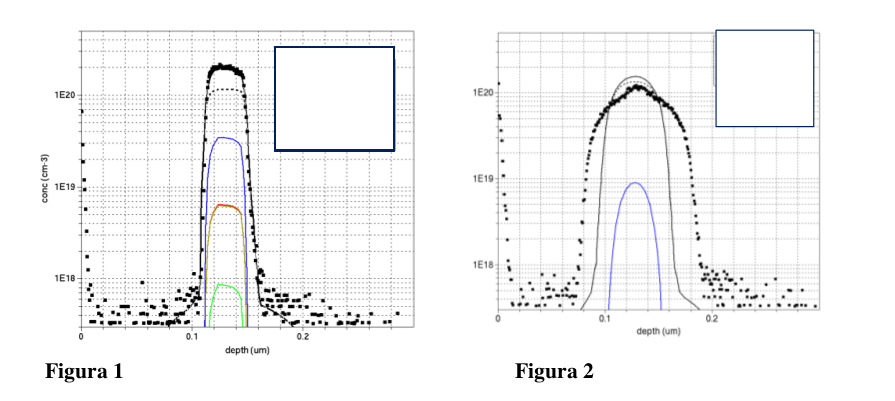
\includegraphics[width=0.5\textwidth]{examfig.png}\\
\raggedright

Il wafer e’ stato poi sottoposto ad un trattamento termico (700 C, 1h ca). Il profilo di As in silicio
osservato e’ riportato nella figura2 (dots neri) e confrontato con le previsioni teoriche di
diffusione (curva nera) basate su un semplice modello “alla Fick”.
{\bf Il modello “alla Fick” sottostima }decimante la diffusione dell’arsenico.
Provare a spiegare qualitativamente il fenomeno, basandosi sui seguenti “indizi”
-La solubilità solida dell’As alla temperatura della crescita epitassiale e’ inferiore a 2E20 cm -3 .
-L’arsenico inattivo in silicio tende a formare cluster As/vacanza

\vspace{3mm}

21/10/09\\

Descrivere una tecnica di {\bf “end point detection”} per attacchi in plasma.
Discutere brevemente di come effetti di {\bf “micro-loading”} possano avere impatto sull’efficacia
della rivelazione dell’ “end point” descritta.

\vspace{3mm}

19/7/10\\

Descrivere, con l’aiuto di disegni, il flusso di processo per realizzare un livello di {\bf metallizzazione in rame},
usando,in luogo della litografia “tradizionale”, tecniche di {\bf  “double patterning”}.

\vspace{3mm}

19/7/10\\

{\bf Channeling effects}

\vspace{3mm}

10/6/10\\

Descrivere brevemente, e con l’aiuto di disegni, il flusso di processo per realizzare {\bf due livelli di
metal ( e relative “vias”) in rame}.

\vspace{3mm}

25/09/15\\

Sia dato un {\bf capacitore MOS} realizzato su un substrato di silicio di tipo p.
Tracciare la caratteristica CV ideale del capacitore i questione, descrivendone
brevemente l’andamento.
1Illustrare come la presenza di trappole all’interfaccia ossido/silicio può modificare la
caratteristica CV.

\vspace{3mm}

25/09/15\\

Descrivere, con l’aiuto di disegni se necessario, almeno due tecniche di {\bf “dimezzamento
del pitch”}, per pattern regolari di linee e spazi. Si illustrino brevemente pro e contro per
ciascuna tecnica illustrata.

\vspace{3mm}

03/7/2009\\

{\bf TED}


